All implementations of the FMM \cite{Ying:2004:JCP, fong2009black, greengard1987fast}, and many fast algorithms for matrix inversion \cite{ambikasaran2014inverse,minden2017recursive, martinsson2005fast, sushnikova2022fmm}, rely on a data structure from computer science called a quadtree in $\mathbb{R}^2$ and an octree in $\mathbb{R}^3$. The defining feature of these data structure is a recursive partition of a bounding box drawn over the region of interest, or ‘root node’, and subdivide it into four equal parts in $\mathbb{R}^2$ and eight equal parts in $\mathbb{R}^3$. These ‘child nodes’ turn are recursively subdivided until a user defined threshold is reached. See figure (\ref{fig:octree_example:sec_1_1}) for an example in $\mathbb{R}^3$. These trees can be `adaptive' by allowing for non-uniform node sizes, and `balanced' to enforce a maximum size constraint between adjacent nodes \cite{sundar2008bottom}.

\begin{figure}
    \centering
    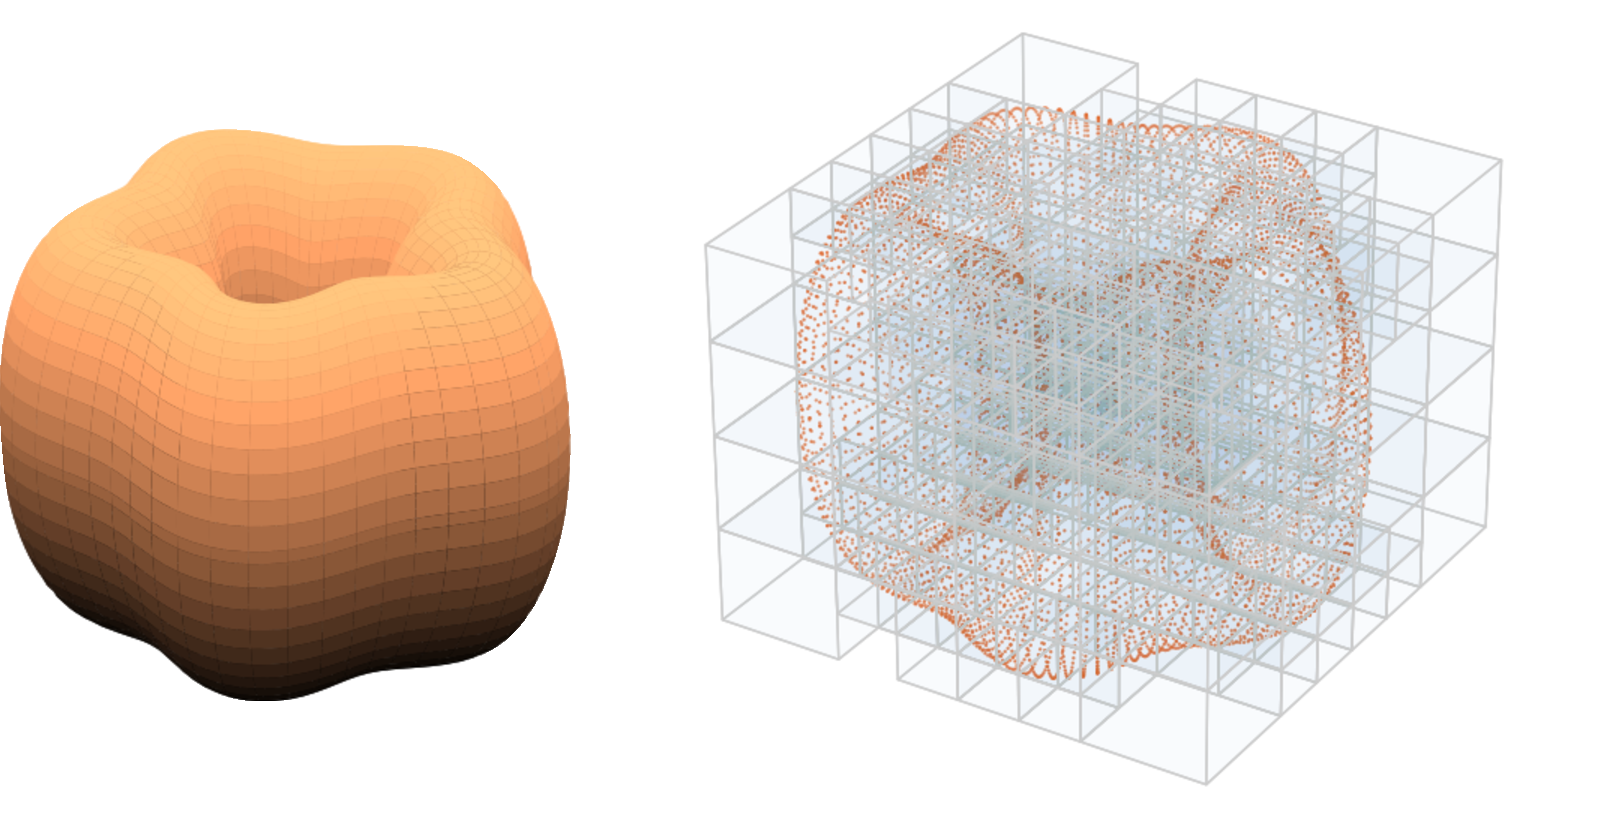
\includegraphics[width=0.7\textwidth]{ch_1/octree_example.pdf}
    \caption{An adaptive octree for random point data placed on the surface of a `wiggly torus' test geometry. The user defines the level of recursion via a threshold for the maximum number of particles in a given node.}
    \label{fig:octree_example:sec_1_1}
\end{figure}

This domain decomposition is behind the power of fast algorithms, as it allows us to hierarchically consider the interactions between different regions of space, which correspond to different nodes. Consider the FMM, 
which consists of two recursions (bottom-up, followed by top-down) of the tree, calculating compressed representations of matrix vector products corresponding to sub-blocks of (\ref{eq:linear_system:sec:1_1}) and applying a low-rank compression when applicable. A full algorithm summary is provided in appendix (\ref{app:a_1_fmm_algorithm}), and we refer to the literature for implementation details and algorithmic analysis \cite{greengard1987fast,fong2009black,Ying:2004:JCP}. Other fast algorithms are similarly structured, emphasising the foundational importance of these tree structures to fast algorithm implementations.

- Note on how we've been deliberately vague on its implementation due to the variety of implementations. 
- Need to have a note on how FMM actually works
- Lead into the main differences between FMM implementations. 
- Sketch out algebraic to analytic tagline, with a note on hierarchical methods.
- Ambikasaran \& Darve summarise differences between different algebraic methods.
%     - H, H2, HSS, HBS, HODLR.


- Comparison of analytical vs algebraic methods
% - Purely algebraic methods
%     - pre-compute and store entire hierarchical matrix.
%     - more storage, more data movement - both vertically and horizontally in memory hierarchy.
% - When the cost of data movement increases faster than arithmetic operations on future architectures, the methods that compute more to store/move less will become advantageous (computationally) - tradeoff results in KIFMM as choice - semi-analytical.


- FMM vs other methods (FFT, Multigrid)
% - Uniform resolution use FFT, introduce FFT as first 'fast algorithm', however has unfavourable communication cost.
% - For non-uniform global problems also have multigrid methods as an alternative, also O(N) cost for elliptic/hyperbolic PDE problems. Gholami, Malhotra, Sundar, Biros (2016) - multigrid decent.


% - algebraic variants commonly argued to be superior as they operate directly on the matrix without the need to pass geometric information
%     - not convincing on their own.
%         - major libraries (PETSc) offer interfaces to insert a matrix free preconditioner as a function, and passing geometric info is something users are willing to do if it increases performance.
%     - Always just comes down to the flops vs bytes trade-off
%     - need a decent reference or description of where architecture technology is heading in order to justify our choice of FMM.

% - Note, analytical FMM have very high arithmetic intensity (flop/byte).
%     - not brute force methods doing wasteful calculations, only doing useful flops. Very different from achieving high arithmetic intensity on dense mat-mat mults or LU decompositions.
%     - Bonsai - an analytical treecode.

% - Fast translation operators crucial - take up a lot of time of the FMM, whatever its implementation.
%     - analytical options for fast translation operators.
%         - Rotation of spherical harmonics 92
%         - Block FFT 36
%         - Planewaves 50

%     - Accelerating M2L step
%         - level-skip M2L method 91
%         - 8,4,2 box method 93
%         - methods that use dual tree traversal alongside multipole acceptance criterion to construct optimal interaction lists 34

%     - Variable expansion order
%         - VFMM 85
%         - Guassian VFMM 20
%         - optimal parameter FMM 28
%     - intuition = boxes further away can afford to be of lower expansion order without loss of accuracy.

%     - Can store translations as matrices - typical optimisation
%         - matrix compression techniques - randomized techniques too.
%         - matrix techniques allow one to take advantage of BLAS
%             - maximises cache utilisation 39 (And US in PyExaFMM)
%         - Combination of techniques like Chebychev with SVD 38
%             - essentially systematic way of doing something like variable expansion order.
% - FMM is a method that has the analytical form to generate small (low-rank) off-diagonal matrices without needing to rely on a numerical approximation method.

% - making better use of translational invariance and rotational symmetry of the interaction list one can reduce the amount of storage further - 30, 32, 89

% - Lay out a sketch of the fast-algorithms for particle summation in terms of the flops/memory trade-off as in Yokota paper.

% - Discuss other hierarchical schemes (H, H2 etc) and explain why FMM is preferred for our application.

% - Explain why our version of FMM - semi-analytical - is preferred for programming.

% - Explain what we can focus on to really accelerate in the semi-analytical FMM to program for exascale, with reference to field translations chapter.

% - Discuss software construction for FMM, and what works and doesn't, what's currently available - and its shortcomings, and positives.

% - Discuss software challenges for high performance FMM, teeing up remaining sections of paper.

% - Close off with alternatives to FMM
% - Allows us to tackle problems that require non-uniform resolution, which isn't possible with the FFT
% - Multigrid methods - link to paper describing their performance.

% $\sim$ 2 pages
